\documentclass[11pt,a4paper]{article}
\usepackage{color}
\usepackage{amsmath, amsthm, amssymb, amsfonts, verbatim}
\usepackage{graphicx}
\usepackage[table,x11names]{xcolor}
\usepackage{geometry}
\title{Assessing glymphatic transport velocities by adjoint methods}

\renewcommand{\comment}[1]{\textcolor{red}{#1}}

\author{Lars Magnus Valnes, Sebastian K. Mitusch, Geir A. Ringstad, Per Kristian Eide, Simon W. Funke, Kent-Andre Mardal }


\begin{document}
\maketitle

\begin{abstract}
\end{abstract}
\section{Introduction}

A novel pathway called the paravascular pathway was discoved in 2011~\cite{iliff2012paravascular} and later found to be particularly active during sleep~\cite{xie2013sleep}. 

It has been proposed that this pathway plays an important role in the waste
clearance of the brain. In particular, since the brain lack a lymphatic system, 
which elsewhere in our body plays a crucial role in waste clearance, the system has been called the glymphatic system~\cite{jessen2015glymphatic}.  
The glymphatic system remains controversial and modeling attempts
has so far mostly failed to explain the biomechanics of the system~\cite{holter2017interstitial, smith2017glymphatic}. A proper biomechanical 
understanding of the pathway has significant potential because
dementia such as Alzheimer´s and Parkinson´s diseases are
associated with accumulation of metabolic waste such as
amyloid-beta and CSF-tau.  
In \cite{ringstad2018brain} brainwide distribution of MRI-contrast was demonstrated during 24 hours after lumbar contrast injection. Brain wide distribution by diffusion alone was deemed unlikely by the authors (some of which are part 
of this study as well). The argument was based on analytical considerations where it was calculated that 50\% contrast enrichment would occur after 
55 hours using the error function which is valid for planar diffusion. However, 
the surface of the brain is folded and is around five times larger than 
a corresponding surface of a ball with the same volume. Hence, 
a more rigorous modeling attempt is warrented. Complicating factors
are however that the contrast in the surrounding CSF is heterogenous
and changes significantly during the 24 hours of the investigations. 
Furthermore, images were obtained only at a few time-points during the investigations in \cite{ringstad2018brain}.  
Our purpose in this paper is to attempt a more rigorous methodology 
for assessing the apparent diffusion process. To this end we employ
adjoint methods to determine the apparent diffusion coefficient 
that would explain the tracer distribution.  
  



\subsection*{Data}
The data consist of a total of 10 MRI observations, including a baseline MRI taken before tracer was injected. The observation points are distributed with 5 observations within 1-2 hours after injection, 1 observation in the timeframes 2-4 hours, 6-9 hours, 24 hours and 48 hours. Figure ~\ref{fig1} shows the distribution of tracers during 24 hours, see also~\cite{ringstad2017glymphatic}.   



\subsection*{Mathematical Model}
In order to assess whether the contrast distribution shown 
in Figure \ref{fig1} is governed by a diffusion process we
aim to solve a PDE constrained optimization problem where
the contrast distribution, boundary conditions, and apparent
diffusion coefficient are solved for by optimizing with
respect to the observed contrast distribution. 
The objective function was defined as 
\begin{equation}
\min_{u,g} F = \quad \sum\limits_i\sp{n} \int\limits_{\Omega} |u(t_i) - u_{obs}(t_i)| \mathrm{d}\Omega + \frac{\alpha}{2} \int\limits_{0}\sp{T} || g ||_{L\sp{2}(\partial\Omega)} \mathrm{d}t + \frac{\beta}{2} \int\limits_{0}\sp{T} || \dot{g} ||_{L\sp{2}(\partial\Omega)}\mathrm{d}t 
\label{EQ::objf}
\end{equation}
subject to   
\begin{equation}
\begin{aligned}
\frac{\partial u}{\partial t} = \nabla \cdot  D_i \nabla u \qquad \text{in} \qquad \Omega \times \left\lbrace 0 , T \right)  \\
u=g(t) \qquad \text{on} \qquad \partial\Omega  \times \left\lbrace 0 , T \right) 
\end{aligned}
\label{Eq::PDE}
\end{equation}
with the domain $\Omega$ contains three sub domains, each with a different diffusion coefficient. We denote the Cerebral Spinal fluid (CSF) domain as $\Omega_1$, the grey matter as $\Omega_2$ and the white matter as $\Omega_3$.

Here $u$ is the contrast distribution, $D_i$ is the apparent diffusion 
coefficient, and $g$ is the boundary condition. Furthermore,  
the domain $\Omega$ contains three sub domains, each with a different diffusion coefficient. We denote the Cerebral Spinal fluid (CSF) domain as $\Omega_1$, the grey matter as $\Omega_2$ and the white matter as $\Omega_3$. The apparent
diffusion constant is assumed constant within the CSF, grey and 
white matter but each region may have different constants.  
The $\alpha$ and $\beta$ parameters are regularization parameters 
and $u_{obs}$ are observations at certain time-points. 
\subsection*{Manufactured Solution}
In order to verify our strategy and test the dependency of the
regularization paramters, we perform a test case with a
known solution.  
The manufactured observations was obtained by forward computation of Eq.\ref{Eq::PDE} with the Dirichlet boundary condition defined as
\begin{equation}
g(t)_{\partial \Omega_1} = 0.3 +0.167t - 0.007t\sp{2} \qquad  0 \leq t \leq 24.
\label{EQ::DIRI}
\end{equation}
The timestep was $dt = 0.02$, and the diffusion coefficients were selected to be 
\begin{equation}
D_{\Omega_1} = 1000 \quad , \quad D_{\Omega_2} = 4.0 \quad , \quad D_{\Omega_3} = 8.0 
\end{equation}  
The magnitude order of the diffusion coefficient are chosen so that they resemble diffusion coefficient in csf, grey and white matter. The forward simulation gave a total of 120 possible observation time points. These points 
will be denoted as $\tau$.

The mesh is patient-specific and was constructed by using the MRI of a patient diagnosed with iNPH. The software Freesurfer was used in segmentation and creating the polyhedral surfaces of the white and grey matter. Then the use of T2 weighted MRI was used to segment the csf compartment surrounding the cerebral. (BrainMesh code accessibility ? ) CGAL[?] was used to combine the polyhedral surfaces and to construed the mesh. The computational requirement for the resulting mesh was significant, therefore a submesh was also constructed, see Fig. ??. 


\section*{Implementation}
The code used the FEniCS project to solve the PDE, using backwards Euler time discretization and first order continuous Galerkin finite elements. The module dolfin adjoint [?] was used to compute the reduced functional, and the optimization used the scipy optimize library to minimize the functional using L-BFGS-B algorithm.   

The implementation used the first observation as initial conditions of Eq.\ref{Eq::PDE}, and for each timestep, the next observation was used as the Dirichlet boundary condition. The Dirichlet boundary condition was imposed on the external boundary for the domain $D_{\Omega_1}$. 


The times in the forward simulation do not always overlap with observations times. Thus a linear interpolation of the forward problem was used to compute the difference from the observation, i.e 
\begin{equation}
u_{linear} = \frac{\Delta t}{dt} U_prev + \frac{dt - \Delta t }{dt} U.
\end{equation}
Here $dt$ is forward timestep and $\Delta t$ is the difference between observation time and forward time. 
The initial values of the optimization algorithm was chosen to be $1,1,1$. Furthermore, to obtain faster convergence in the optimization, the diffusion coefficients was scaled to have the same magnitude, i.e.  $D_{\Omega_1}$ was scaled, so that $D_{\Omega_1} = D\sp {s}_{\Omega_1}100$.     


The noise susceptibility was also tested by adding an uniform distribution noise term to the observations. The noise term was constructed using numpy random and multiplied with a noise amplitude. The noise amplitudes were chosen to be $ 10\%, 50\%, 100\%$ of the maximum initial boundary conditions, so that negative concentrations are avoided.  

The real data observations had observation times that had an unevenly distribution over 24 hours. Thus having  constant time between observations is not realsitic. Therefore the number of observation and the unevenly distribution of them will be tested. To accurately depict the real data observations. 



\section*{Non-linear relation}
The MR images are provided by Oslo University Hospital Rikshospitalet and can be seen in Fig.??. The software Freesurfer was used to segment and align each of the observations, which made it possible to estimate voxelwise intensity increase. The tracer causes the longitudinal(spin-lattice) relaxation time $T_{1}$ to shorten with the following relation
\begin{equation}
\frac{1}{T_{1}\sp{c}} = \frac{1}{T_{1}\sp{0}} + r_{1}*C .
\label{EQ::contrast}
\end{equation}
The superscripts indicating with contrast and without contrast and $r_1$ as the relaxivity constant for the MRI-contrast in a medium. The relation between intensity and the relaxation time is non-linear, and is expressed with the following equations. The signal intensity $SI$ of the sequence is given by
\begin{equation}
SI = M_{n} \sin \theta e\sp{ - TE/T_2\sp{*} },
\label{EQ::SI_T2}
\end{equation}
with  $TE$ and $\theta$ respectively denoting the echo time and the flip angle. Also $T2\sp{*}$ is transverse magnetization caused by a combination of spin-spin relaxation and magnetic field inhomogeneity. It is defined as 
\begin{equation}
\frac{1}{T_2\sp{*}} = \frac{1}{T_2} + \gamma \Delta B_{in} ,
\end{equation}
with $T2$ transverse (spin-spin) relaxation time, $\gamma$ is the gyromagnetic ratio and $\Delta B_{in}$ is the magnetic field inhomogeneity across a voxel. The expression can be simplified by neglecting the $T2$ term in the signal, since $TE <<T_2\sp{*}$ for this MRI sequence. Thus Eq. \ref{EQ::SI_T2} becomes 
\begin{equation}
SI = M_{n} \sin \theta.
\label{EQ::SI}
\end{equation}
In article [?], the term $M_n$ is defined as the magnetization for the n-echo 
\begin{equation}
M_{n} = M_{0}  \left[ (1-\beta)\frac{(1-(\alpha \beta)\sp{n-1} }{1-\alpha\beta} + (\alpha \beta)\sp{n-1}(1-\gamma) + \gamma ( \alpha \beta)\sp{n-1} \frac{M_{e}}{M_{0}}  \right]   
\end{equation}
with 
\begin{equation}
\frac{M_{e}}{M_{0}} = - \left[ \frac{ 1 -\delta + \alpha \delta (1-\beta ) \frac{1-\alpha\beta\sp{m}}{1-\alpha \beta} + \alpha\delta(\alpha\beta)\sp{m-1} - \alpha\sp{m}\rho}{1 +\rho \alpha\sp{m} } \right].
\end{equation}
Using the following definitions
\begin{equation}
\begin{aligned}
\alpha &= \cos ( \theta ) \\
\beta  &= e\sp{- \sp{T_b}/_{T_1}\sp{0} } \\
\delta &= e\sp{- \sp{T_a}/_{T_1}\sp{0} } \\
\gamma &= e\sp{- \sp{T_w}/_{T_1}\sp{0} } \\
\rho   &= e\sp{- \sp{TR}/_{T_1}\sp{0} }  \\
T_w    &= TR - T_a -T_b(m-1)       .\\
\end{aligned}
\end{equation}
Here $T_b$ is known as the echo spacing, $T_a$ is the inversion time, $T_w$ the time delay, $TR$ as the repetition time, $m$ is the number of echo spacings and $T1$ is the longitudinal(spin-lattice) relaxation time for a given medium. The $M_0$ is a calibration constant of the magnetization. The center echo denoted as $n=\sp{m}/_2$ will be the signal that we will consider when estimating MRI-contrast. Given Eq.\ref{EQ::SI} we have that relative intensity increase can be written as 
\begin{equation}
\frac{SI\sp{c}}{SI\sp{0}} = \frac{ M_{n}\sp{c} \sin (\theta)}{ M_{n}\sp{0} \sin (\theta) } ,
\end{equation}
We define that  
\begin{equation}
f(T_1) = M_{n}/M_{0} ,
\label{FIG::F}
\end{equation}
which gives the following relation 
\begin{equation}
\frac{f(T_{1}\sp{c} ) }{f(T_{1}\sp{0})}  = \frac{SI\sp{c}}{SI\sp{0}} 
\end{equation}
Thus we can express the $T_1$ change due to contrast as 
\begin{equation}
f ( T_{1}\sp{c} ) = \frac{SI\sp{c}}{SI\sp{0}} f(T_{1}\sp{0}) 
\end{equation}
and we can then estimate concentration using Eq.\ref{EQ::contrast} if we know $T_{1}\sp{0}$. The $T_{1}\sp{0}$ was obtained using MRI.


 


The convergence of L-BFGS-B algorithm can be seen in Fig.??. 
\begin{itemize}
\item describe the imaging, shortly with ref to JCI  
\item describe the abstract mathematical problem to be solved, ie. PDE constrained opt problem where we 
address coefficients and bc  
\item the details: finite element, reduced problem, BFGS,  
\end{itemize}

\begin{figure}
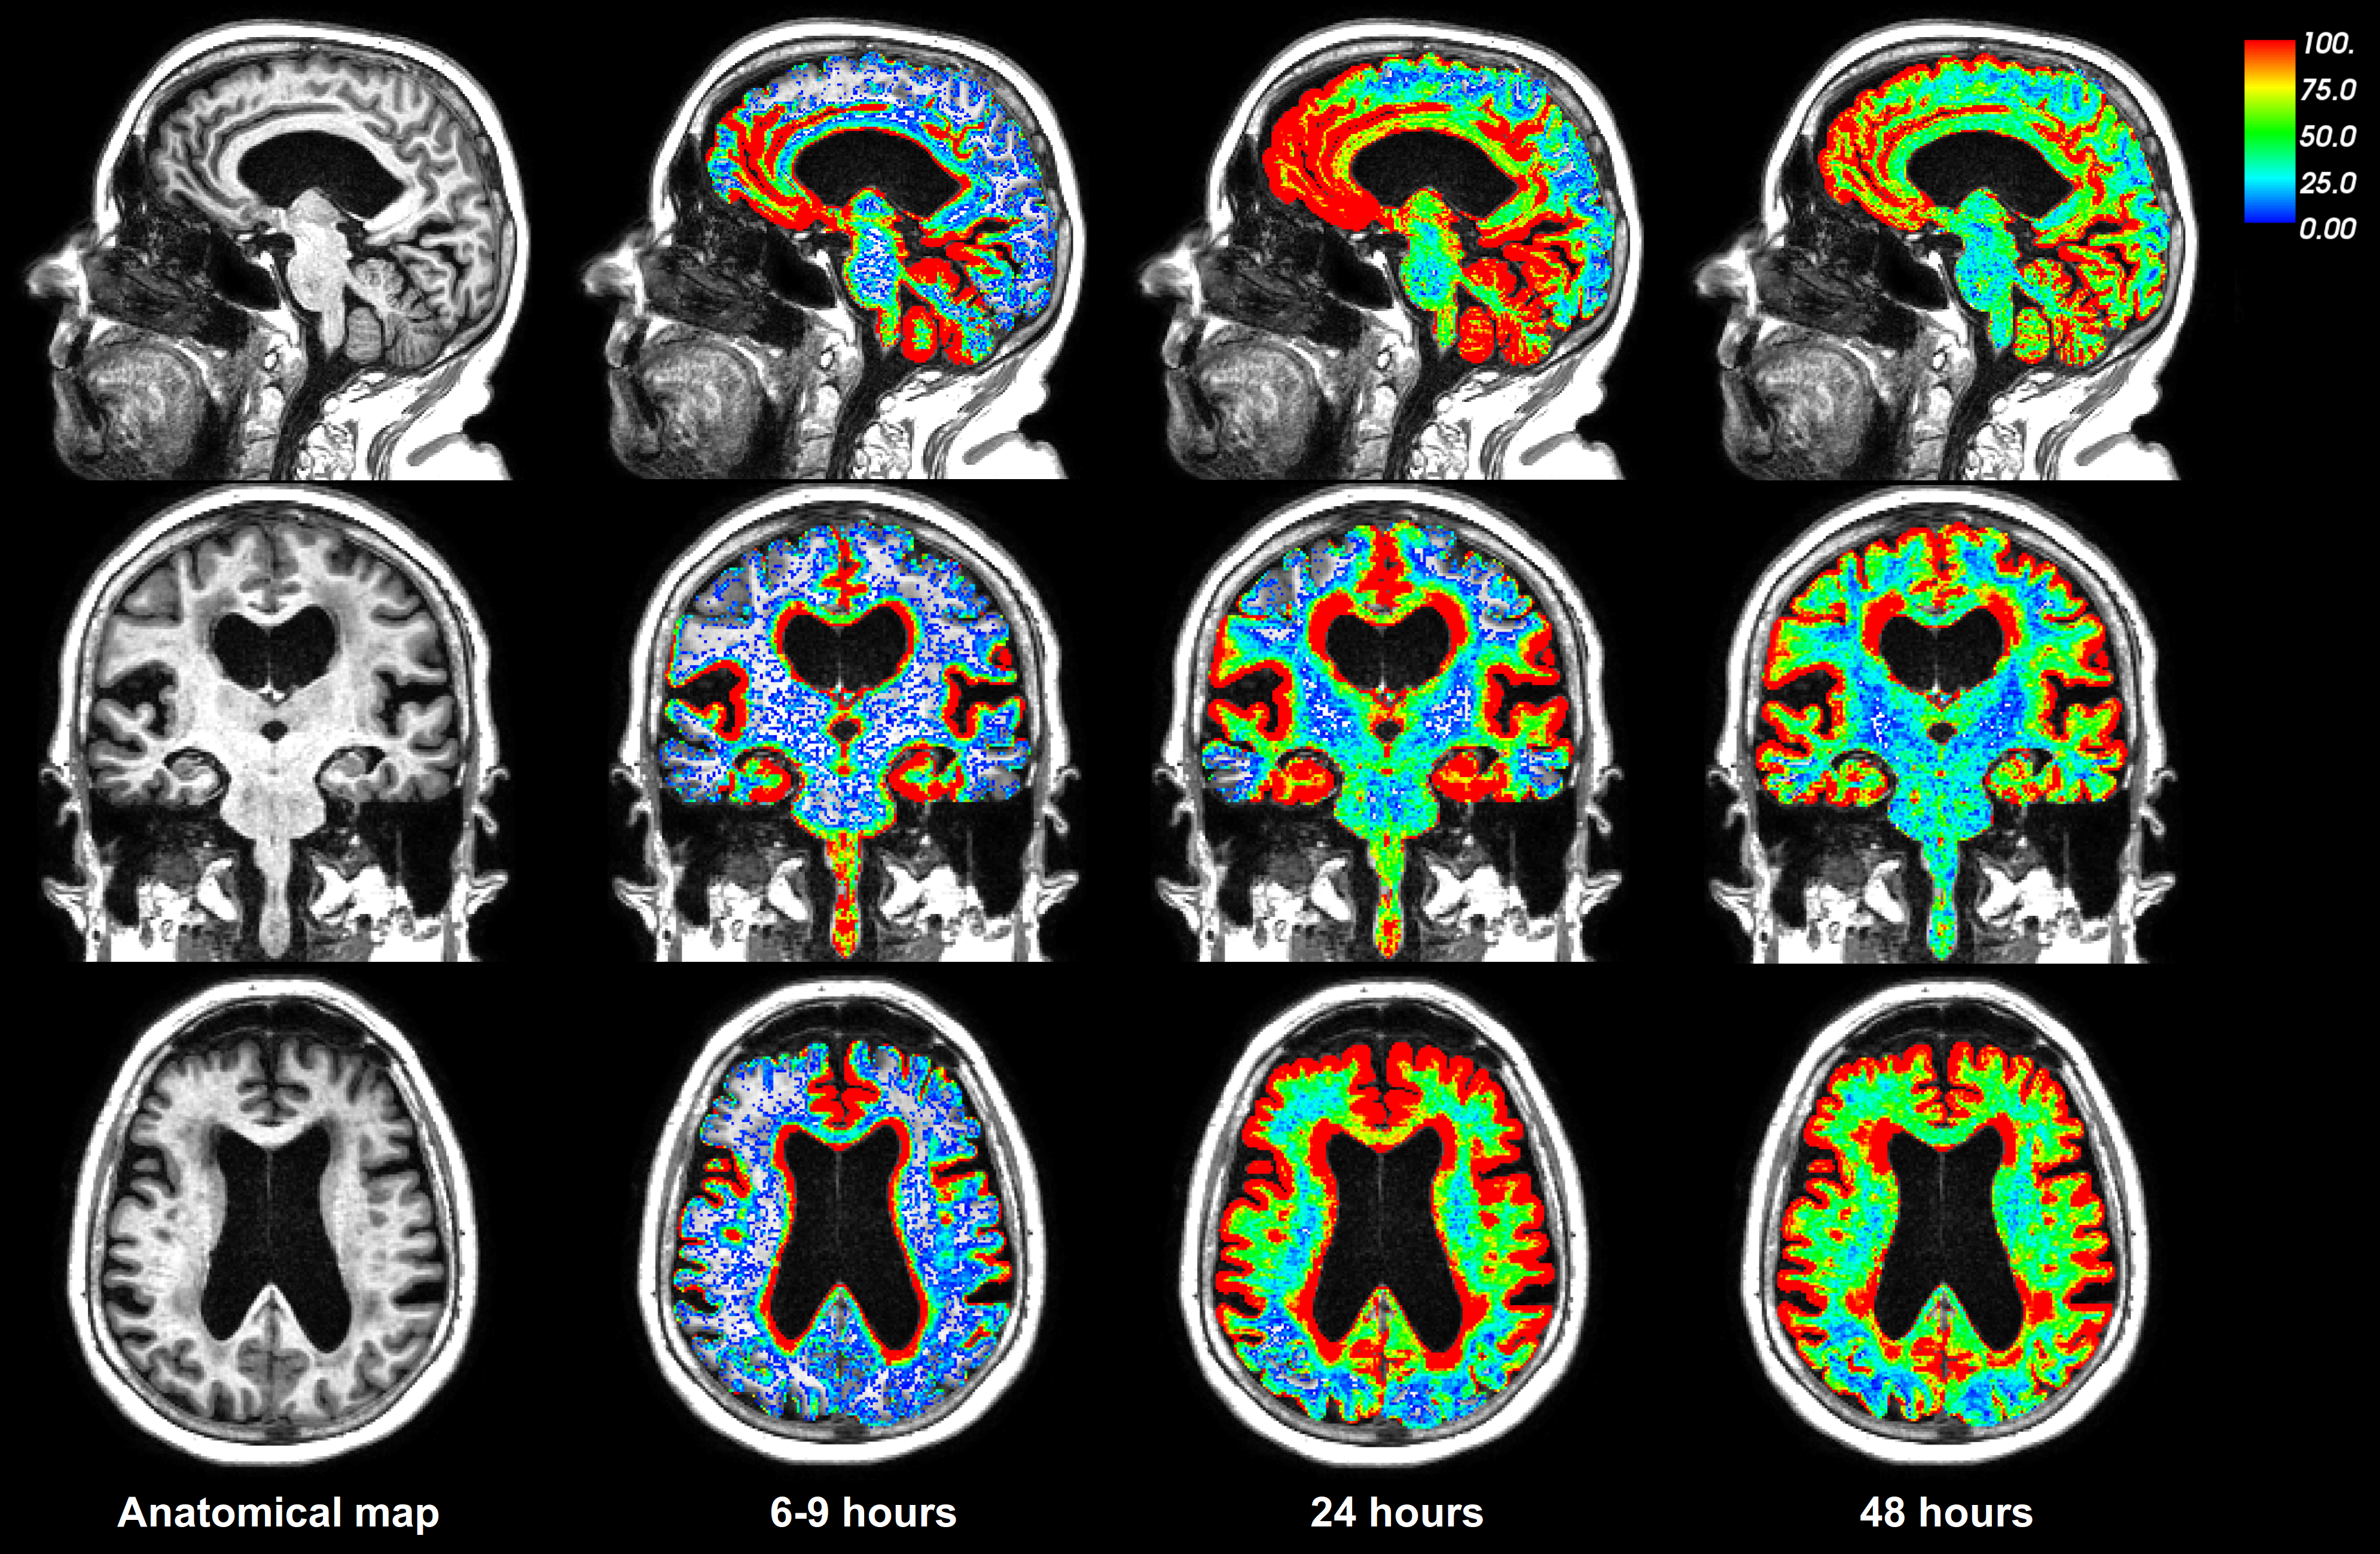
\includegraphics[width=0.95\textwidth]{PatID-68-new-100.png} 
\label{fig1} 
\caption{Shows the percentage intensity increase from baseline at different observation times. }
\end{figure}

\begin{figure}
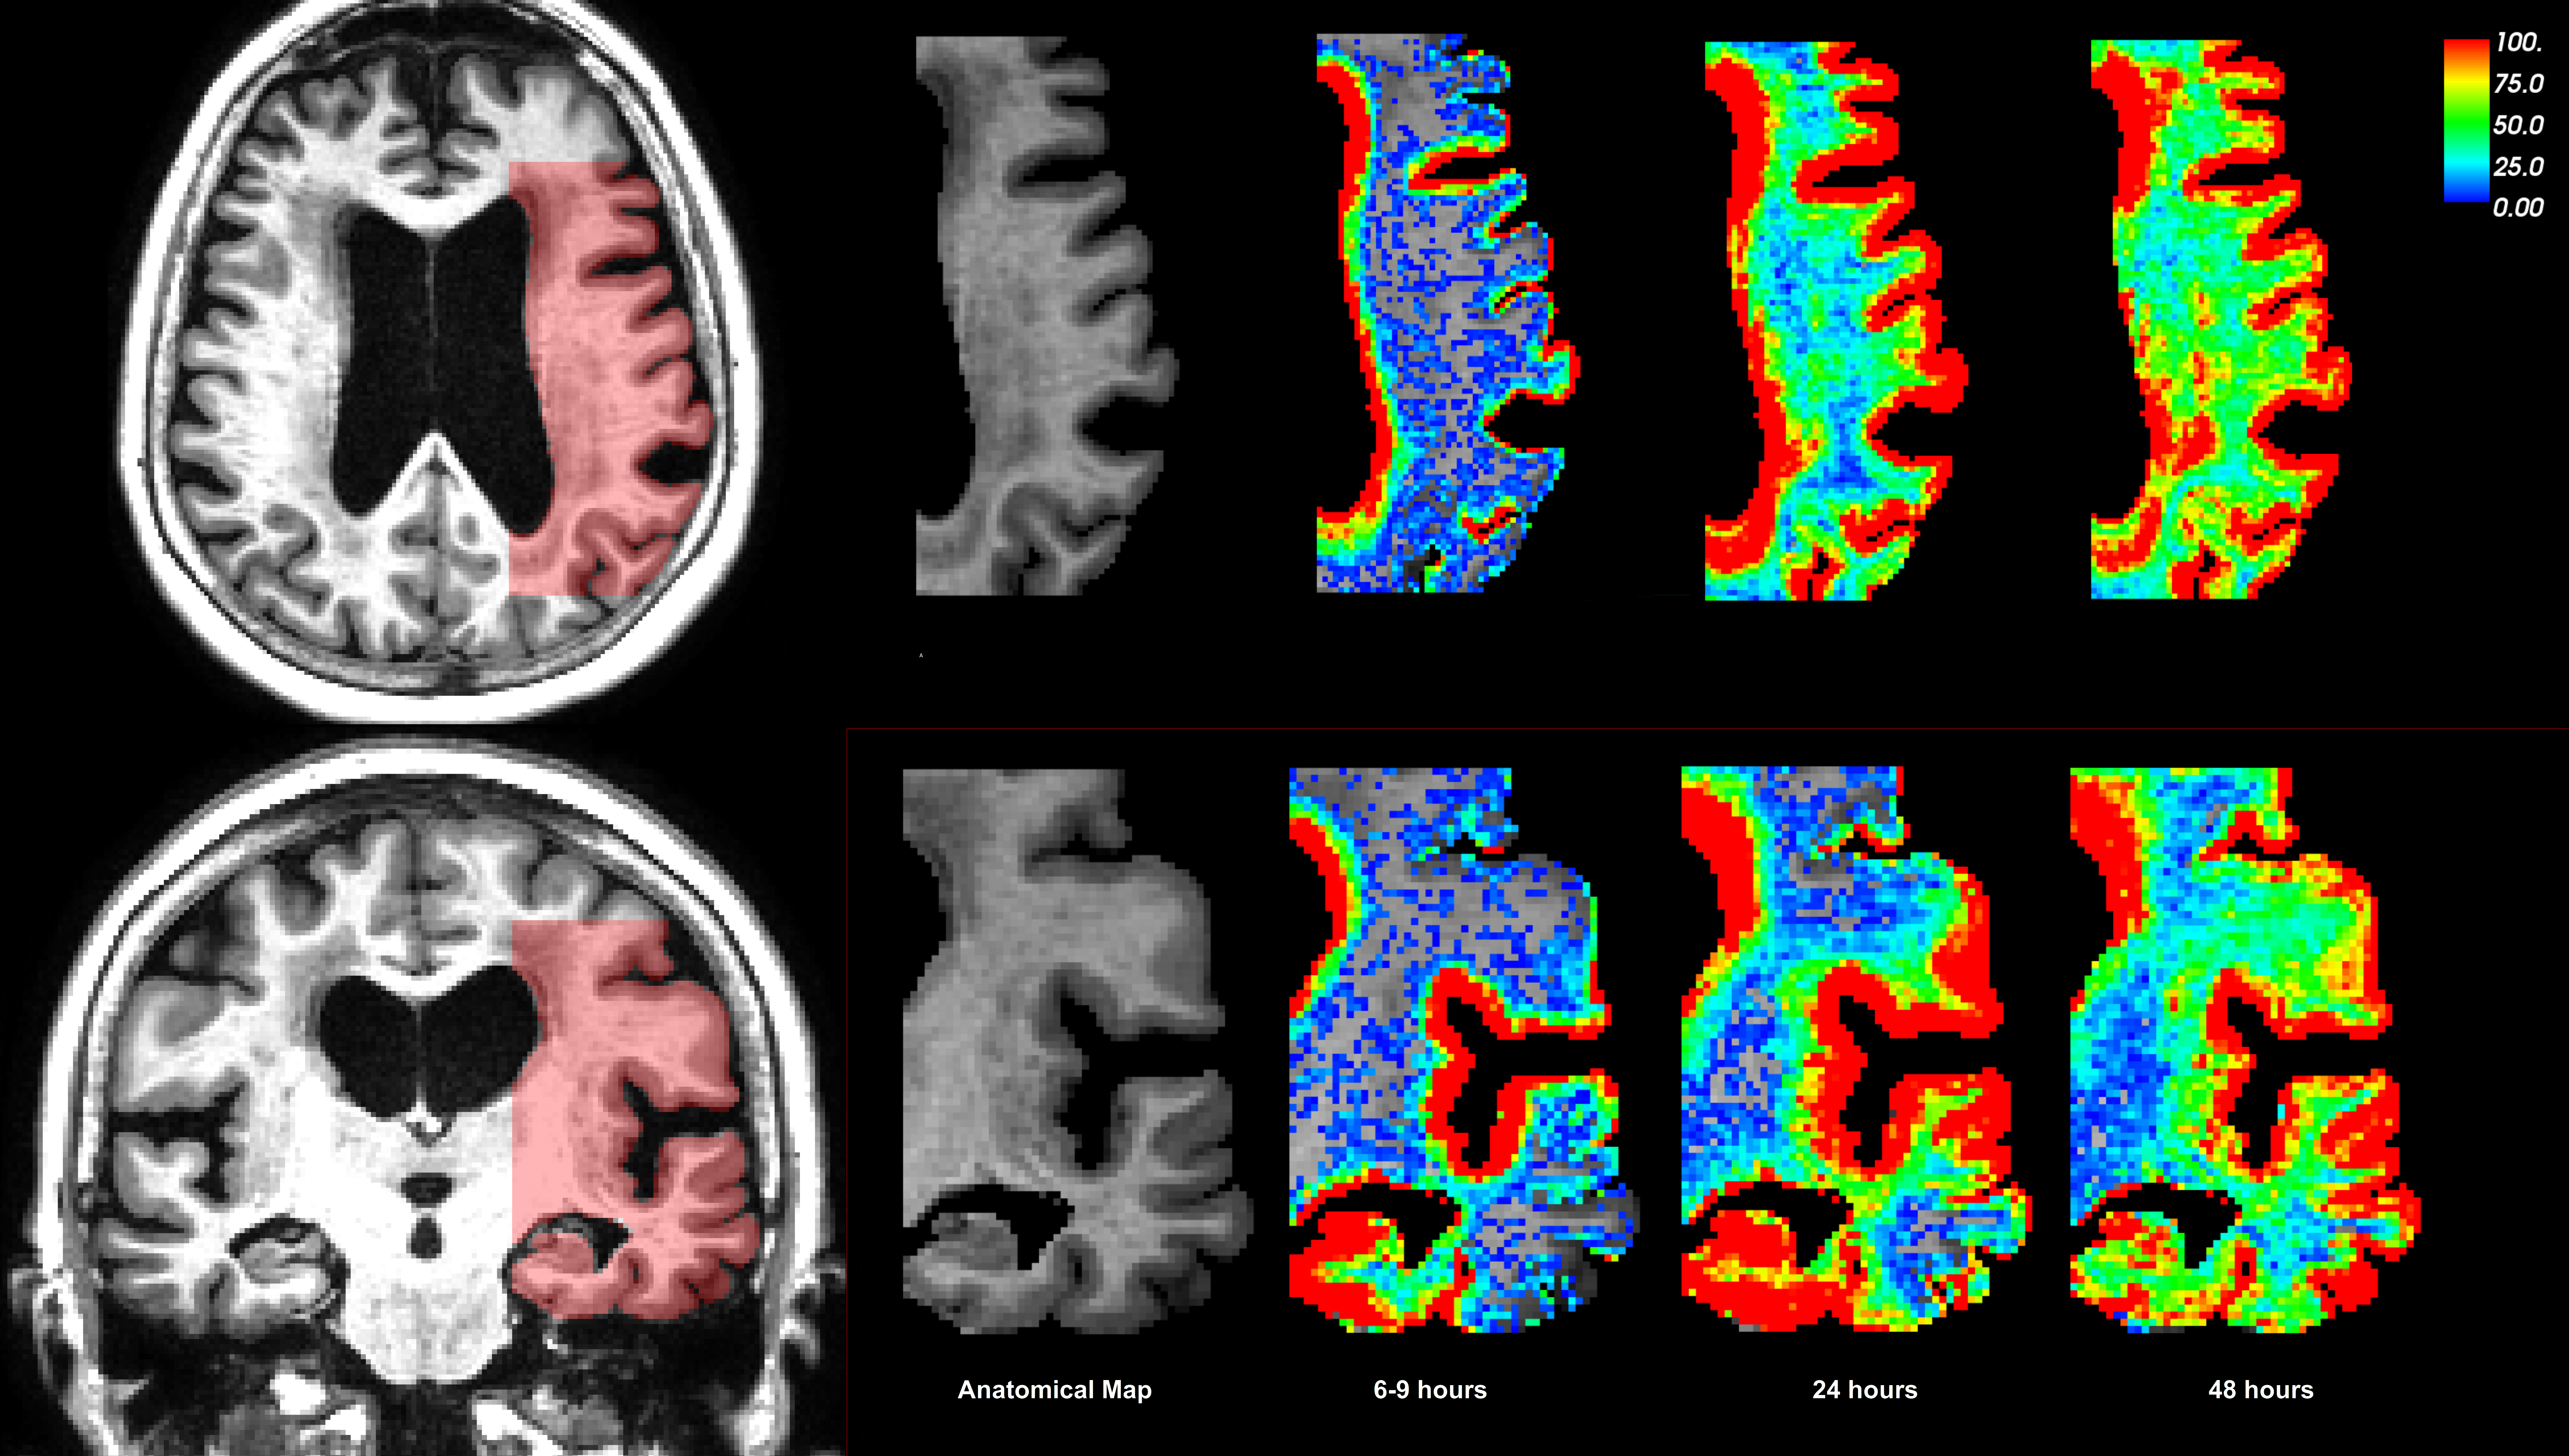
\includegraphics[width=0.95\textwidth]{Zoom-PatID-68.png} 
\label{fig1} 
\caption{Shows the percentage intensity increase from baseline at different observation times in the area corresponding to the generated mesh that is marked red in the left panel.}
\end{figure}

\begin{figure}
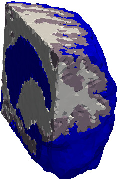
\includegraphics[width=0.3\textwidth]{mesh-eps-converted-to.pdf} 
\label{fig1} 
\caption{Shows the mesh created from the baseline MR image with 3 domains. ( wrap ?? ) }
\end{figure}


\section{Results}
\begin{itemize}
\item 2D experiments as have already been done (with and without noise/ with and without observations everywhere in time) 
\item 2D experiments should highlight the impact of the regularization parameter wrt number of iterations and diffusion 
coeff 
\item 3D experiments based on data generated  
\item 3D experiments based on real data (\comment{lars: we need to try testing this}) 
\end{itemize}

\subsection{The relaxation parameters}
The relaxation parameters needs to be calibrated depending on the problem, and thus the diffusion parameters were computed by large range of relaxation parameters values. The results are shown in Tab.\ref{Tab::1}, and it is shown in red that $\alpha=1.0$ have large discrepancy in the parameters values of $D_{\Omega_1}$. 



\subsection{The number of timessteps}
The first results focus on the accuracy of the minimization based on the number of time steps. It can be assumed that the error decreases  while the number of time steps increases since the Dirichlet boundary condition in Eq.\ref{EQ::DIRI} are quadratic, while the forward problem is a linear approximation. 

This can be seen in Tab.??, Tab.??





In Tab.\ref{Tab::1}, we can see that the 

\subsection{The number of observations}
The number of observations can also be considered an important aspect, since the number of observations can be limited. Thus the number of observations set to $5,10 $ and $20$, and  



\subsection{The noise susceptibility}

The noise susceptibility can be seen in Tab. ?? and Tab. ??, and we see that a noise amplitude of $10 \%$ does not lead to significant change 




\section{Discussion}



The diffusion equation does not pose any difficulties numerically 


This method can be adapted to 


\newpage 
\newgeometry{top=0.5cm}

\begin{table}
\centering
\caption{Shows the relaxation parameters $\alpha$ and $\beta$, number of timesteps $k$ and number of observation $\tau$ with the resulting number of iterations and estimated optimal parameters for the diffusion coefficients. }
\resizebox{0.9\textwidth}{!}{\begin{tabular}{*{8}c}
$\alpha$ & $\beta$ & k  & iter & $ D_{\Omega_1} = 1000$ & $ D_{\Omega_2} = 4.0 $ & $D_{\Omega_3} = 8.0 $ & $g$ \\
\hline
\rowcolor{red}  1.0e+00 	 & 1.0e+00 	 & 10 & 225 	 & +4.148 & +0.304 & +0.092 & +0.135 \\ 
\rowcolor{red}  1.0e+00 	 & 1.0e-01 	 & 10 & 206 	 & +4.272 & +0.305 & +0.091 & +0.142 \\ 
\rowcolor{red}  1.0e+00 	 & 1.0e-02 	 & 10 & 233 	 & +4.272 & +0.305 & +0.091 & +0.143 \\ 
\rowcolor{red}  1.0e+00 	 & 1.0e-03 	 & 10 & 208 	 & +4.437 & +0.305 & +0.091 & +0.143 \\ 
\rowcolor{red}  1.0e+00 	 & 1.0e-04 	 & 10 & 204 	 & +4.271 & +0.306 & +0.091 & +0.143 \\ 
\rowcolor{red}  1.0e+00 	 & 1.0e-05 	 & 10 & 203 	 & +4.400 & +0.305 & +0.091 & +0.143 \\ 
\rowcolor{red}  1.0e+00 	 & 1.0e-06 	 & 10 & 222 	 & +4.584 & +0.304 & +0.090 & +0.143 \\
 
 1.0e-01 	 & 1.0e+00 	 & 10 & 207 	 & +0.127 & +0.093 & +0.041 & +0.027 \\ 
 1.0e-01 	 & 1.0e-01 	 & 10 & 196 	 & +0.121 & +0.093 & +0.041 & +0.046 \\ 
 1.0e-01 	 & 1.0e-02 	 & 10 & 232 	 & +0.123 & +0.093 & +0.041 & +0.056 \\ 
 1.0e-01 	 & 1.0e-03 	 & 10 & 183 	 & +0.122 & +0.093 & +0.040 & +0.057 \\ 
 1.0e-01 	 & 1.0e-04 	 & 10 & 212 	 & +0.122 & +0.093 & +0.040 & +0.057 \\ 
 1.0e-01 	 & 1.0e-05 	 & 10 & 168 	 & +0.122 & +0.093 & +0.041 & +0.057 \\
 1.0e-01 	 & 1.0e-06 	 & 10 & 195 	 & +0.122 & +0.093 & +0.041 & +0.057 \\ 

 1.0e-02 	 & 1.0e+00 	 & 10 & 227 	 & +0.015 & +0.067 & +0.039 & +0.018 \\ 
 1.0e-02 	 & 1.0e-01 	 & 10 & 153 	 & +0.006 & +0.065 & +0.039 & +0.021 \\ 
 1.0e-02 	 & 1.0e-02 	 & 10 & 184 	 & +0.005 & +0.065 & +0.039 & +0.039 \\ 
 1.0e-02 	 & 1.0e-03 	 & 10 & 176 	 & +0.004 & +0.065 & +0.039 & +0.048 \\ 
 1.0e-02 	 & 1.0e-04 	 & 10 & 195 	 & +0.005 & +0.065 & +0.039 & +0.049 \\ 
 1.0e-02 	 & 1.0e-05 	 & 10 & 215 	 & +0.004 & +0.065 & +0.039 & +0.051 \\ 
 1.0e-02 	 & 1.0e-06 	 & 10 & 205 	 & +0.005 & +0.065 & +0.039 & +0.050 \\ 

 1.0e-03 	 & 1.0e+00 	 & 10 & 179 	 & +0.004 & +0.064 & +0.039 & +0.019 \\ 
 1.0e-03 	 & 1.0e-01 	 & 10 & 221 	 & -0.005 & +0.063 & +0.039 & +0.018 \\ 
 1.0e-03 	 & 1.0e-02 	 & 10 & 89 	 & -0.007 & +0.063 & +0.039 & +0.026 \\ 
 1.0e-03 	 & 1.0e-03 	 & 10 & 77 	 & -0.005 & +0.062 & +0.039 & +0.027 \\ 
 1.0e-03 	 & 1.0e-04 	 & 10 & 100 	 & -0.006 & +0.062 & +0.039 & +0.027 \\ 
 1.0e-03 	 & 1.0e-05 	 & 10 & 105 	 & -0.006 & +0.062 & +0.039 & +0.027 \\ 
 1.0e-03 	 & 1.0e-06 	 & 10 & 123 	 & -0.007 & +0.062 & +0.039 & +0.028 \\ 


 1.0e-04 	 & 1.0e+00 	 & 10 & 236 	 & +0.004 & +0.063 & +0.039 & +0.019 \\ 
 1.0e-04 	 & 1.0e-01 	 & 10 & 195 	 & -0.006 & +0.062 & +0.039 & +0.018 \\ 
 1.0e-04 	 & 1.0e-02 	 & 10 & 152 	 & -0.006 & +0.062 & +0.039 & +0.022 \\ 
 1.0e-04 	 & 1.0e-03 	 & 10 & 119 	 & -0.008 & +0.062 & +0.039 & +0.026 \\ 
 1.0e-04 	 & 1.0e-04 	 & 10 & 106 	 & -0.007 & +0.062 & +0.039 & +0.026 \\ 
 1.0e-04 	 & 1.0e-05 	 & 10 & 109 	 & -0.007 & +0.062 & +0.039 & +0.026 \\ 
 1.0e-04 	 & 1.0e-06 	 & 10 & 99 	 & -0.008 & +0.062 & +0.039 & +0.026 \\
 
 1.0e-05 	 & 1.0e+00 	 & 10 & 139 	 & +0.004 & +0.063 & +0.039 & +0.019 \\ 
 1.0e-05 	 & 1.0e-01 	 & 10 & 170 	 & -0.006 & +0.062 & +0.039 & +0.018 \\ 
 1.0e-05 	 & 1.0e-02 	 & 10 & 182 	 & -0.007 & +0.062 & +0.039 & +0.020 \\ 
 1.0e-05 	 & 1.0e-03 	 & 10 & 70 	 & -0.007 & +0.062 & +0.039 & +0.026 \\ 
 1.0e-05 	 & 1.0e-04 	 & 10 & 77 	 & -0.007 & +0.062 & +0.039 & +0.026 \\ 
 1.0e-05 	 & 1.0e-05 	 & 10 & 104 	 & -0.008 & +0.062 & +0.039 & +0.026 \\ 
 1.0e-05 	 & 1.0e-06 	 & 10 & 92 	 & -0.007 & +0.062 & +0.039 & +0.026 \\ 

 1.0e-06 	 & 1.0e+00 	 & 10 & 163 	 & +0.003 & +0.064 & +0.039 & +0.019 \\ 
 1.0e-06 	 & 1.0e-01 	 & 10 & 218 	 & -0.006 & +0.062 & +0.039 & +0.018 \\ 
 1.0e-06 	 & 1.0e-02 	 & 10 & 134 	 & -0.008 & +0.062 & +0.039 & +0.023 \\ 
 1.0e-06 	 & 1.0e-03 	 & 10 & 79 	 & -0.006 & +0.062 & +0.039 & +0.026 \\ 
 1.0e-06 	 & 1.0e-04 	 & 10 & 107 	 & -0.007 & +0.062 & +0.039 & +0.026 \\ 
 1.0e-06 	 & 1.0e-05 	 & 10 & 103 	 & -0.008 & +0.062 & +0.039 & +0.026 \\ 
 1.0e-06 	 & 1.0e-06 	 & 10 & 91 	 & -0.008 & +0.062 & +0.039 & +0.026 \\  
\end{tabular}}
\label{Tab::1}
\end{table} 







\newpage
\begin{table}
\centering
\caption{Shows the relaxation parameters $\alpha$ and $\beta$, number of timesteps $k$, the resulting number of iterations, the relative error of the estimated optimal parameters for the diffusion coefficients and the relative error for $g$. The noise amplitude was set to 0.03, and $\tau =[2.4, 4.8, 7.2, 9.6, 12.0, 14.4, 16.8, 19.2, 21.6, 24.0]$ }
\resizebox{0.8\textwidth}{!}{\begin{tabular}{*{8}c}
$\alpha$ & $\beta$ & k  & iter & $ D_{\Omega_1} $ & $ D_{\Omega_2} $ & $D_{\Omega_3} $ & wrong $g$ \\
\hline
 1.0e+00 	 & 1.0e+00 	 & 10 & 218 	 & +4.266 & +0.304 & +0.092 & +0.135 \\ 
 1.0e+00 	 & 1.0e-01 	 & 10 & 223 	 & +4.565 & +0.304 & +0.090 & +0.142 \\ 
 1.0e+00 	 & 1.0e-02 	 & 10 & 199 	 & +4.268 & +0.305 & +0.090 & +0.143 \\ 
 1.0e+00 	 & 1.0e-03 	 & 10 & 222 	 & +4.274 & +0.305 & +0.090 & +0.143 \\ 
 1.0e+00 	 & 1.0e-04 	 & 10 & 211 	 & +4.448 & +0.306 & +0.090 & +0.143 \\ 
 1.0e+00 	 & 1.0e-05 	 & 10 & 227 	 & +4.527 & +0.304 & +0.090 & +0.143 \\ 
 1.0e+00 	 & 1.0e-06 	 & 10 & 263 	 & +4.266 & +0.306 & +0.091 & +0.143 \\ 
 
 1.0e-01 	 & 1.0e+00 	 & 10 & 167 	 & +0.131 & +0.093 & +0.041 & +0.027 \\ 
 1.0e-01 	 & 1.0e-01 	 & 10 & 195 	 & +0.125 & +0.093 & +0.039 & +0.046 \\ 
 1.0e-01 	 & 1.0e-02 	 & 10 & 218 	 & +0.126 & +0.093 & +0.040 & +0.056 \\ 
 1.0e-01 	 & 1.0e-03 	 & 10 & 161 	 & +0.129 & +0.094 & +0.040 & +0.057 \\ 
 1.0e-01 	 & 1.0e-04 	 & 10 & 180 	 & +0.135 & +0.092 & +0.042 & +0.057 \\ 
 1.0e-01 	 & 1.0e-05 	 & 10 & 169 	 & +0.123 & +0.093 & +0.041 & +0.057 \\ 
 1.0e-01 	 & 1.0e-06 	 & 10 & 201 	 & +0.119 & +0.093 & +0.040 & +0.057 \\ 

 1.0e-02 	 & 1.0e+00 	 & 10 & 183 	 & +0.013 & +0.067 & +0.040 & +0.018 \\ 
 1.0e-02 	 & 1.0e-01 	 & 10 & 149 	 & +0.002 & +0.066 & +0.038 & +0.021 \\ 
 1.0e-02 	 & 1.0e-02 	 & 10 & 185 	 & -0.005 & +0.065 & +0.040 & +0.040 \\ 
 1.0e-02 	 & 1.0e-03 	 & 10 & 213 	 & +0.004 & +0.066 & +0.038 & +0.049 \\ 
 1.0e-02 	 & 1.0e-04 	 & 10 & 151 	 & +0.008 & +0.066 & +0.039 & +0.047 \\ 
 1.0e-02 	 & 1.0e-05 	 & 10 & 197 	 & +0.004 & +0.064 & +0.040 & +0.051 \\ 
 1.0e-02 	 & 1.0e-06 	 & 10 & 185 	 & +0.012 & +0.063 & +0.038 & +0.049 \\ 

 1.0e-03 	 & 1.0e+00 	 & 10 & 183 	 & +0.007 & +0.062 & +0.038 & +0.019 \\ 
 1.0e-03 	 & 1.0e-01 	 & 10 & 181 	 & -0.011 & +0.063 & +0.039 & +0.019 \\ 
 1.0e-03 	 & 1.0e-02 	 & 10 & 122 	 & -0.008 & +0.063 & +0.040 & +0.025 \\ 
 1.0e-03 	 & 1.0e-03 	 & 10 & 158 	 & -0.004 & +0.062 & +0.040 & +0.028 \\ 
 1.0e-03 	 & 1.0e-04 	 & 10 & 168 	 & -0.013 & +0.063 & +0.038 & +0.029 \\ 
 1.0e-03 	 & 1.0e-05 	 & 10 & 120 	 & -0.010 & +0.063 & +0.040 & +0.028 \\ 
 1.0e-03 	 & 1.0e-06 	 & 10 & 132 	 & -0.002 & +0.062 & +0.039 & +0.028 \\ 

 1.0e-04 	 & 1.0e+00 	 & 10 & 176 	 & +0.000 & +0.063 & +0.039 & +0.019 \\ 
 1.0e-04 	 & 1.0e-01 	 & 10 & 180 	 & -0.001 & +0.062 & +0.039 & +0.019 \\ 
 1.0e-04 	 & 1.0e-02 	 & 10 & 120 	 & +0.000 & +0.063 & +0.039 & +0.024 \\ 
 1.0e-04 	 & 1.0e-03 	 & 10 & 119 	 & -0.004 & +0.062 & +0.039 & +0.026 \\ 
 1.0e-04 	 & 1.0e-04 	 & 10 & 77 	 & -0.005 & +0.061 & +0.038 & +0.027 \\ 
 1.0e-04 	 & 1.0e-05 	 & 10 & 104 	 & -0.004 & +0.062 & +0.038 & +0.027 \\ 
 1.0e-04 	 & 1.0e-06 	 & 10 & 109 	 & -0.007 & +0.062 & +0.039 & +0.027 \\ 

 1.0e-05 	 & 1.0e+00 	 & 10 & 220 	 & +0.005 & +0.063 & +0.039 & +0.019 \\ 
 1.0e-05 	 & 1.0e-01 	 & 10 & 193 	 & -0.009 & +0.062 & +0.039 & +0.019 \\ 
 1.0e-05 	 & 1.0e-02 	 & 10 & 163 	 & -0.013 & +0.063 & +0.039 & +0.021 \\ 
 1.0e-05 	 & 1.0e-03 	 & 10 & 115 	 & -0.007 & +0.063 & +0.040 & +0.026 \\ 
 1.0e-05 	 & 1.0e-04 	 & 10 & 82 	 & -0.007 & +0.062 & +0.038 & +0.027 \\ 
 1.0e-05 	 & 1.0e-05 	 & 10 & 145 	 & -0.001 & +0.062 & +0.039 & +0.027 \\ 
 1.0e-05 	 & 1.0e-06 	 & 10 & 147 	 & -0.012 & +0.061 & +0.040 & +0.027 \\ 

 1.0e-06 	 & 1.0e+00 	 & 10 & 138 	 & +0.002 & +0.063 & +0.039 & +0.019 \\ 
 1.0e-06 	 & 1.0e-01 	 & 10 & 184 	 & -0.006 & +0.063 & +0.039 & +0.019 \\ 
 1.0e-06 	 & 1.0e-02 	 & 10 & 83 	 & -0.006 & +0.063 & +0.040 & +0.025 \\ 
 1.0e-06 	 & 1.0e-03 	 & 10 & 91 	 & -0.013 & +0.063 & +0.039 & +0.026 \\ 
 1.0e-06 	 & 1.0e-04 	 & 10 & 109 	 & -0.005 & +0.062 & +0.038 & +0.027 \\ 
 1.0e-06 	 & 1.0e-05 	 & 10 & 116 	 & -0.007 & +0.063 & +0.039 & +0.027 \\ 
 1.0e-06 	 & 1.0e-06 	 & 10 & 108 	 & +0.001 & +0.062 & +0.040 & +0.027 \\ 
\end{tabular}}
\label{Tab::4}
\end{table} 
\begin{table}[t]
\centering
\caption{Shows the relaxation parameters $\alpha$ and $\beta$, number of timesteps $k$, the resulting number of iterations, the relative error of the estimated optimal parameters for the diffusion coefficients and the relative error for $g$. The noise amplitude was set to 0.3, and $\tau =[2.4, 4.8, 7.2, 9.6, 12.0, 14.4, 16.8, 19.2, 21.6, 24.0]$  }
\resizebox{0.8\textwidth}{!}{\begin{tabular}{*{8}c}
$\alpha$ & $\beta$ & k  & iter & $ D_{\Omega_1} $ & $ D_{\Omega_2} $ & $D_{\Omega_3} $ & $g$ \\
\hline
 1.0e+00 	 & 1.0e+00 	 & 10 & 212 	 & +4.268 & +0.310 & +0.073 & +0.138 \\ 
 1.0e+00 	 & 1.0e-01 	 & 10 & 211 	 & +4.122 & +0.302 & +0.085 & +0.146 \\ 
 1.0e+00 	 & 1.0e-02 	 & 10 & 221 	 & +4.773 & +0.298 & +0.089 & +0.147 \\ 
 1.0e+00 	 & 1.0e-03 	 & 10 & 257 	 & +4.872 & +0.301 & +0.090 & +0.147 \\ 
 1.0e+00 	 & 1.0e-04 	 & 10 & 238 	 & +4.186 & +0.293 & +0.097 & +0.148 \\ 
 1.0e+00 	 & 1.0e-05 	 & 10 & 204 	 & +4.251 & +0.313 & +0.085 & +0.147 \\ 
 1.0e+00 	 & 1.0e-06 	 & 10 & 223 	 & +4.493 & +0.310 & +0.085 & +0.147 \\ 
 1.0e-01 	 & 1.0e+00 	 & 10 & 145 	 & +0.126 & +0.100 & +0.054 & +0.035 \\ 
 1.0e-01 	 & 1.0e-01 	 & 10 & 199 	 & +0.115 & +0.125 & +0.026 & +0.060 \\ 
 1.0e-01 	 & 1.0e-02 	 & 10 & 217 	 & +0.128 & +0.092 & +0.036 & +0.071 \\ 
 1.0e-01 	 & 1.0e-03 	 & 10 & 242 	 & +0.109 & +0.093 & +0.031 & +0.073 \\ 
 1.0e-01 	 & 1.0e-04 	 & 10 & 275 	 & +0.187 & +0.094 & +0.028 & +0.073 \\ 
 1.0e-01 	 & 1.0e-05 	 & 10 & 237 	 & +0.048 & +0.099 & +0.039 & +0.073 \\ 
 1.0e-01 	 & 1.0e-06 	 & 10 & 225 	 & +0.092 & +0.111 & +0.055 & +0.073 \\ 
 1.0e-02 	 & 1.0e+00 	 & 10 & 208 	 & +0.017 & +0.075 & +0.037 & +0.029 \\ 
 1.0e-02 	 & 1.0e-01 	 & 10 & 199 	 & -0.013 & +0.068 & +0.046 & +0.040 \\ 
 1.0e-02 	 & 1.0e-02 	 & 10 & 348 	 & -0.043 & +0.073 & +0.041 & +0.063 \\ 
 1.0e-02 	 & 1.0e-03 	 & 10 & 400 	 & +0.056 & +0.058 & +0.031 & +0.075 \\ 
 1.0e-02 	 & 1.0e-04 	 & 10 & 393 	 & -0.050 & +0.088 & +0.044 & +0.077 \\ 
 1.0e-02 	 & 1.0e-05 	 & 10 & 359 	 & +0.022 & +0.068 & +0.027 & +0.076 \\ 
 1.0e-02 	 & 1.0e-06 	 & 10 & 369 	 & +0.001 & +0.074 & +0.024 & +0.076 \\ 
 1.0e-03 	 & 1.0e+00 	 & 10 & 207 	 & -0.001 & +0.065 & +0.051 & +0.029 \\ 
 1.0e-03 	 & 1.0e-01 	 & 10 & 280 	 & +0.028 & +0.051 & +0.053 & +0.038 \\ 
 1.0e-03 	 & 1.0e-02 	 & 10 & 565 	 & -0.059 & +0.076 & +0.033 & +0.053 \\ 
 \rowcolor{orange} 1.0e-03 	 & 1.0e-03 	 & 10 & 673 	 & -0.035 & +0.066 & +0.032 & +0.108 \\ 
 \rowcolor{orange} 1.0e-03 	 & 1.0e-04 	 & 10 & 604 	 & -0.026 & +0.061 & +0.049 & +0.182 \\ 
 \rowcolor{orange} 1.0e-03 	 & 1.0e-05 	 & 10 & 666 	 & +0.012 & +0.070 & +0.038 & +0.182 \\ 
 \rowcolor{orange} 1.0e-03 	 & 1.0e-06 	 & 10 & 893 	 & +0.027 & +0.070 & +0.022 & +0.180 \\ 
 1.0e-04 	 & 1.0e+00 	 & 10 & 204 	 & +0.015 & +0.062 & +0.043 & +0.030 \\ 
 1.0e-04 	 & 1.0e-01 	 & 10 & 269 	 & +0.005 & +0.057 & +0.037 & +0.038 \\ 
 1.0e-04 	 & 1.0e-02 	 & 10 & 559 	 & -0.072 & +0.067 & +0.044 & +0.050 \\ 
\rowcolor{orange} 1.0e-04 	 & 1.0e-03 	 & 10 & 691 	 & -0.023 & +0.055 & +0.040 & +0.175 \\ 
\rowcolor{red}  1.0e-04 	 & 1.0e-04 	 & 10 & 1001 	 & -0.012 & +0.066 & +0.030 & +0.745 \\ 
\rowcolor{red}  1.0e-04 	 & 1.0e-05 	 & 10 & 1001 	 & +0.038 & +0.057 & +0.034 & +1.113 \\ 
\rowcolor{red} 1.0e-04 	 & 1.0e-06 	 & 10 & 1001 	 & +0.015 & +0.063 & +0.035 & +1.127 \\ 
 1.0e-05 	 & 1.0e+00 	 & 10 & 184 	 & -0.025 & +0.076 & +0.041 & +0.029 \\ 
 1.0e-05 	 & 1.0e-01 	 & 10 & 357 	 & -0.011 & +0.070 & +0.052 & +0.038 \\ 
 1.0e-05 	 & 1.0e-02 	 & 10 & 399 	 & +0.041 & +0.075 & +0.042 & +0.049 \\ 
 \rowcolor{orange} 1.0e-05 	 & 1.0e-03 	 & 10 & 689 	 & +0.044 & +0.062 & +0.020 & +0.172 \\ 
\rowcolor{red} 1.0e-05 	 & 1.0e-04 	 & 10 & 915 	 & +0.030 & +0.077 & +0.039 & +1.027 \\ 
\rowcolor{red} 1.0e-05 	 & 1.0e-05 	 & 10 & 1001 	 & +0.017 & +0.061 & +0.045 & +1.953 \\ 
\rowcolor{red}  1.0e-05 	 & 1.0e-06 	 & 10 & 1001 	 & -0.018 & +0.071 & +0.045 & +2.545 \\ 
 1.0e-06 	 & 1.0e+00 	 & 10 & 177 	 & +0.060 & +0.069 & +0.039 & +0.029 \\ 
 1.0e-06 	 & 1.0e-01 	 & 10 & 302 	 & +0.011 & +0.039 & +0.039 & +0.038 \\ 
 1.0e-06 	 & 1.0e-02 	 & 10 & 457 	 & +0.011 & +0.055 & +0.036 & +0.050 \\ 
\rowcolor{orange} 1.0e-06 	 & 1.0e-03 	 & 10 & 738 	 & -0.022 & +0.055 & +0.042 & +0.172 \\ 
\rowcolor{red}  1.0e-06 	 & 1.0e-04 	 & 10 & 1001 	 & -0.043 & +0.042 & +0.054 & +1.180 \\ 
\rowcolor{red}  1.0e-06 	 & 1.0e-05 	 & 10 & 1001 	 & +0.006 & +0.052 & +0.033 & +3.365 \\ 
\rowcolor{red}  1.0e-06 	 & 1.0e-06 	 & 10 & 1001 	 & -0.002 & +0.065 & +0.051 & +3.402 \\ 
\end{tabular}}
\label{Tab::5}
\end{table} 



\begin{table}
\centering
\caption{ $\tau = [4.8, 9.6, 14.4, 19.2, 24.0]$}
\resizebox{\textwidth}{!}{\begin{tabular}{*{8}c}
$\alpha$ & $\beta$ & k & iter & $ D_{\Omega_1} = 1000$ & $ D_{\Omega_2} = 4.0 $ & $D_{\Omega_3} = 8.0 $ \\
\hline
 1.0e-04 	 & 1.0e+00 	 & 10 & 161 	 & +0.081 & +0.027 & +0.049 & +0.023 \\ 
 1.0e-04 	 & 1.0e-01 	 & 10 & 185 	 & +0.123 & +0.046 & +0.037 & +0.021 \\ 
 1.0e-04 	 & 1.0e-02 	 & 10 & 265 	 & +0.160 & +0.082 & +0.033 & +0.016 \\ 
 1.0e-05 	 & 1.0e+00 	 & 10 & 192 	 & +0.083 & +0.026 & +0.049 & +0.023 \\ 
 1.0e-05 	 & 1.0e-01 	 & 10 & 223 	 & +0.118 & +0.047 & +0.037 & +0.020 \\ 
 1.0e-05 	 & 1.0e-02 	 & 10 & 267 	 & +0.159 & +0.084 & +0.033 & +0.016 \\ 
 1.0e-06 	 & 1.0e+00 	 & 10 & 176 	 & +0.082 & +0.026 & +0.049 & +0.023 \\ 
 1.0e-06 	 & 1.0e-01 	 & 10 & 229 	 & +0.120 & +0.046 & +0.037 & +0.021 \\ 
 1.0e-06 	 & 1.0e-02 	 & 10 & 253 	 & +0.156 & +0.080 & +0.033 & +0.018 \\ 
 1.0e-04 	 & 1.0e+00 	 & 20 & 202 	 & +0.007 & -0.050 & +0.017 & +0.028 \\ 
 1.0e-04 	 & 1.0e-01 	 & 20 & 336 	 & +0.028 & -0.009 & +0.009 & +0.023 \\
 1.0e-04 	 & 1.0e-02 	 & 20 & 320 	 & +0.025 & +0.025 & +0.015 & +0.013 \\ 
 1.0e-05 	 & 1.0e+00 	 & 20 & 195 	 & +0.007 & -0.051 & +0.017 & +0.029 \\ 
 1.0e-05 	 & 1.0e-01 	 & 20 & 320 	 & +0.029 & -0.011 & +0.009 & +0.026 \\ 
 1.0e-05 	 & 1.0e-02 	 & 20 & 351 	 & +0.023 & +0.017 & +0.011 & +0.019 \\ 
 1.0e-06 	 & 1.0e+00 	 & 20 & 224 	 & +0.007 & -0.051 & +0.017 & +0.029 \\ 
 1.0e-06 	 & 1.0e-01 	 & 20 & 334 	 & +0.027 & -0.012 & +0.009 & +0.026 \\ 
 1.0e-06 	 & 1.0e-02 	 & 20 & 340 	 & +0.020 & +0.016 & +0.012 & +0.019 \\ 
 1.0e-04 	 & 1.0e+00 	 & 40 & 308 	 & -0.032 & -0.081 & +0.002 & +0.031 \\ 
 1.0e-04 	 & 1.0e-01 	 & 40 & 379 	 & -0.004 & -0.033 & -0.006 & +0.026 \\ 
 1.0e-04 	 & 1.0e-02 	 & 40 & 377 	 & +0.006 & +0.006 & -0.001 & +0.008 \\ 
 1.0e-05 	 & 1.0e+00 	 & 40 & 212 	 & -0.034 & -0.083 & +0.001 & +0.031 \\ 
 1.0e-05 	 & 1.0e-01 	 & 40 & 396 	 & -0.007 & -0.036 & -0.006 & +0.028 \\ 
 1.0e-05 	 & 1.0e-02 	 & 40 & 374 	 & +0.009 & +0.007 & -0.003 & +0.014 \\ 
 1.0e-06 	 & 1.0e+00 	 & 40 & 226 	 & -0.034 & -0.082 & +0.001 & +0.031 \\ 
 1.0e-06 	 & 1.0e-01 	 & 40 & 313 	 & -0.007 & -0.037 & -0.006 & +0.030 \\ 
 1.0e-06 	 & 1.0e-02 	 & 40 & 368 	 & +0.006 & +0.006 & -0.004 & +0.013 \\ 
\end{tabular}}
\end{table} 

\begin{table}
\centering
\caption{ Shows the $\tau = [1.2, 2.4, 3.6, 4.8, 6.0, 7.2, 8.4, 9.6, 10.8, 12.0, 13.2, 14.4, 15.6, 16.8, 17.0, 19.2, 20.4, 21.6, 22.8, 24.0] $}
\resizebox{\textwidth}{!}{\begin{tabular}{*{8}c}
$\alpha$ & $\beta$ & k & iter & $ D_{\Omega_1} = 1000$ & $ D_{\Omega_2} = 4.0 $ & $D_{\Omega_3} = 8.0 $ \\
\hline
 1.0e-04 	 & 1.0e+00 	 & 10 & 246 	 & -0.046 & +0.038 & +0.023 & +0.031 \\ 
 1.0e-04 	 & 1.0e-01 	 & 10 & 292 	 & -0.052 & +0.038 & +0.024 & +0.032 \\ 
 1.0e-04 	 & 1.0e-02 	 & 10 & 338 	 & -0.053 & +0.038 & +0.024 & +0.032 \\ 
 1.0e-05 	 & 1.0e+00 	 & 10 & 290 	 & -0.047 & +0.038 & +0.023 & +0.031 \\ 
 1.0e-05 	 & 1.0e-01 	 & 10 & 316 	 & -0.052 & +0.038 & +0.024 & +0.032 \\ 
 1.0e-05 	 & 1.0e-02 	 & 10 & 389 	 & -0.052 & +0.038 & +0.024 & +0.033 \\ 
 1.0e-06 	 & 1.0e+00 	 & 10 & 282 	 & -0.047 & +0.038 & +0.023 & +0.031 \\ 
 1.0e-06 	 & 1.0e-01 	 & 10 & 308 	 & -0.052 & +0.038 & +0.024 & +0.032 \\ 
 1.0e-06 	 & 1.0e-02 	 & 10 & 285 	 & -0.052 & +0.038 & +0.024 & +0.032 \\ 
 1.0e-04 	 & 1.0e+00 	 & 20 & 228 	 & -0.008 & +0.016 & +0.009 & +0.006 \\ 
 1.0e-04 	 & 1.0e-01 	 & 20 & 331 	 & -0.001 & +0.018 & +0.006 & +0.006 \\ 
 1.0e-04 	 & 1.0e-02 	 & 20 & 367 	 & +0.003 & +0.018 & +0.005 & +0.007 \\ 
 1.0e-05 	 & 1.0e+00 	 & 20 & 194 	 & -0.008 & +0.016 & +0.009 & +0.006 \\ 
 1.0e-05 	 & 1.0e-01 	 & 20 & 312 	 & -0.001 & +0.018 & +0.006 & +0.006 \\ 
 1.0e-05 	 & 1.0e-02 	 & 20 & 266 	 & +0.004 & +0.018 & +0.005 & +0.007 \\ 
 1.0e-06 	 & 1.0e+00 	 & 20 & 179 	 & -0.008 & +0.016 & +0.009 & +0.006 \\ 
 1.0e-06 	 & 1.0e-01 	 & 20 & 245 	 & -0.002 & +0.018 & +0.006 & +0.006 \\ 
 1.0e-06 	 & 1.0e-02 	 & 20 & 362 	 & +0.003 & +0.018 & +0.005 & +0.007 \\ 
 1.0e-04 	 & 1.0e+00 	 & 40 & 279 	 & -0.007 & +0.000 & +0.003 & +0.002 \\ 
 1.0e-04 	 & 1.0e-01 	 & 40 & 313 	 & +0.004 & +0.003 & +0.000 & +0.002 \\ 
 1.0e-04 	 & 1.0e-02 	 & 40 & 273 	 & +0.017 & +0.006 & -0.001 & +0.001 \\ 
 1.0e-05 	 & 1.0e+00 	 & 40 & 238 	 & -0.007 & +0.000 & +0.002 & +0.002 \\ 
 1.0e-05 	 & 1.0e-01 	 & 40 & 317 	 & +0.004 & +0.003 & +0.000 & +0.002 \\ 
 1.0e-05 	 & 1.0e-02 	 & 40 & 336 	 & +0.015 & +0.005 & -0.001 & +0.001 \\ 
 1.0e-06 	 & 1.0e+00 	 & 40 & 261 	 & -0.007 & +0.000 & +0.002 & +0.002 \\ 
 1.0e-06 	 & 1.0e-01 	 & 40 & 318 	 & +0.004 & +0.003 & +0.000 & +0.002 \\ 
 1.0e-06 	 & 1.0e-02 	 & 40 & 375 	 & +0.015 & +0.005 & -0.001 & +0.001 \\ 
\end{tabular}}
\end{table} 



\begin{table}
\centering
\caption{$\tau = [0.8, 1.0, 1.2, 1.8, 2.4, 3.6, 5.4, 7.6, 24.0] $ noise 0.0}
\resizebox{\textwidth}{!}{\begin{tabular}{*{8}c}
$\alpha$ & $\beta$ & k & iter & $ D_{\Omega_1} = 1000$ & $ D_{\Omega_2} = 4.0 $ & $D_{\Omega_3} = 8.0 $ \\
 1.0e-04 	 & 1.0e+00 	 & 40 & 517 	 & -0.034 & -0.006 & -0.022 & +0.058 \\ 
 1.0e-04 	 & 1.0e-01 	 & 40 & 660 	 & -0.045 & -0.013 & -0.024 & +0.052 \\ 
 1.0e-04 	 & 1.0e-02 	 & 40 & 283 	 & -0.059 & -0.020 & -0.027 & +0.331 \\ 
 1.0e-05 	 & 1.0e+00 	 & 40 & 588 	 & -0.034 & -0.006 & -0.022 & +0.060 \\ 
 1.0e-05 	 & 1.0e-01 	 & 40 & 686 	 & -0.046 & -0.013 & -0.024 & +0.067 \\ 
 1.0e-05 	 & 1.0e-02 	 & 40 & 400 	 & -0.059 & -0.020 & -0.027 & +0.260 \\ 
 1.0e-06 	 & 1.0e+00 	 & 40 & 618 	 & -0.034 & -0.006 & -0.022 & +0.058 \\ 
 1.0e-06 	 & 1.0e-01 	 & 40 & 826 	 & -0.046 & -0.013 & -0.024 & +0.070 \\ 
 1.0e-06 	 & 1.0e-02 	 & 40 & 632 	 & -0.058 & -0.020 & -0.027 & +0.183 \\ 

\end{tabular}}
\label{Tab::1}
\end{table} 
\begin{table}
\centering
\caption{$\tau = [0.8, 1.0, 1.2, 1.8, 2.4, 3.6, 5.4, 7.6, 24.0] $ noise 0.3}
\resizebox{\textwidth}{!}{\begin{tabular}{*{8}c}
$\alpha$ & $\beta$ & k & iter & $ D_{\Omega_1} = 1000$ & $ D_{\Omega_2} = 4.0 $ & $D_{\Omega_3} = 8.0 $ \\
\hline
 1.0e-04 	 & 1.0e+00 	 & 40 & 519 	 & +0.003 & +0.029 & +0.035 & +0.067 \\ 
 1.0e-04 	 & 1.0e-01 	 & 40 & 653 	 & -0.096 & +0.015 & +0.016 & +0.070 \\ 
\rowcolor{red}  1.0e-04 	 & 1.0e-02 	 & 40 & 575 	 & -0.050 & -0.001 & +0.057 & +0.281 \\ 
 1.0e-05 	 & 1.0e+00 	 & 40 & 585 	 & -0.050 & -0.007 & +0.017 & +0.068 \\ 
 1.0e-05 	 & 1.0e-01 	 & 40 & 871 	 & -0.023 & +0.024 & +0.019 & +0.079 \\ 
\rowcolor{red}  1.0e-05 	 & 1.0e-02 	 & 40 & 466 	 & -0.045 & +0.042 & +0.019 & +0.281 \\ 
 1.0e-06 	 & 1.0e+00 	 & 40 & 584 	 & -0.045 & +0.019 & +0.006 & +0.071 \\ 
 1.0e-06 	 & 1.0e-01 	 & 40 & 546 	 & +0.005 & +0.019 & -0.001 & +0.079 \\ 
\rowcolor{red}  1.0e-06 	 & 1.0e-02 	 & 40 & 648 	 & -0.074 & -0.008 & +0.041 & +0.227 \\ 
\end{tabular}}
\label{Tab::1}
\end{table} 




In Tab. ?? we observe that the optimal relaxation parameters are found for $\alpha := \lbrace 1.e-4 1.e-5 1.e-6 \rbrace$ and $\beta := \lbrace 1.0 0.1 0.01 \rbrace$. This will be the region of interest for the relaxation parameters.

The dependency on number of timesteps can be seen in Fig.??.






\bibliographystyle{amsplain}
\bibliography{references}


\end{document}


